\documentclass{article}
\usepackage{graphicx}
\usepackage{amsfonts}
\usepackage{url}
\usepackage{pdfpages}
\usepackage{amsmath,amssymb}
\usepackage{enumerate}
\usepackage{color}
\usepackage{amsthm,amsmath}
\usepackage{bbm}
\usepackage{mhchem}

%for stacking below a sum or max...
\usepackage{mathtools}

\usepackage[colorlinks]{hyperref}

\newcommand{\comment}[2]{\vspace{0.6cm}{\bf Comment:} {\it #1.}

\vspace{0.3cm}{\bf Answer:} #2}

\begin{document}
\title{Response to Referee Comments: Parallel Adaptive Importance Sampling}
\maketitle
First of all, we would like to thank the referees and the associate editor for
their time in reading and commenting on our manuscript. We thank all of you and Professor Higdon for your patience in waiting for these delayed corrections. In this document
we will address each of the points raised, and describe any relevant
changes that have been made to the paper. We have made several substantial changes, including the renaming of the algorithm and paper from ``parallel adaptive importance sampling'' (PAIS) to ``ensemble transport adaptive importance sampling'' (ETAIS). We have also replaced two of the numerical examples. In particular we have incorporated a new bimodal example with differing scales in the two modes, and for which we have tested the ETAIS with three different resampling algorithms. This in particular we feel makes the paper stronger, and we hope that the referees and editors will now agree that the paper is ready for publication.

\section*{Referee 1 comments}

\comment{This is supposed to be a parallel algorithm and yet it's implemention is serial. Furthermore, the authors don't seem to be entirely sure that parallelization will work since they comment that it's effectiveness will depend on various factors. The title seems somehow misleading to me. Maybe if the "parallel" part of the title is removed and the discussion about parallelization is treated as a possibility instead of a critical part of the algorithm, then the document will be less confusing.}{Despite the fact that we felt that we had demonstrated the feasibility of the parallelisation of this method, we agree with the referee that we have not demonstrated this in the numerics. Furthermore, this algorithm delivers a speed-up even when run in serial. As such, we are happy to change the name of the algorithm to ``Ensemble Transport Adaptive Importance Sampling'' (ETAIS). This required some rewriting throughout the paper. In particular, we have toned down the emphasis on parallelisation, and put more emphasis on the fact that this algorithm also delivers speed-up for serial implementations. See the second paragraph of the discussion.}

\comment{Also, the comparison between serial PAIS and the naive parallel MCMC is strange if there is no parallelization.}{Most of the numerics compares our methodology to Metropolis-Hastings, based on the number of likelihood evaluations required, rather than runtime, with the argument being based on the idea that this approach is most suitable for targets with expensive likelihood evaluations. Since the only difference between implementations in parallel or serial of our method will be in CPU runtime (due to extra overheads due to communications between processors), it is still valid for us to compare to a naively parallelised Metropolis-Hastings approach, since our choice of serial/parallel implementation makes no difference to these results. For the final example where we consider runtime, a sentence has been added to state that our results will be slightly overoptimistic based on the lack of communication overheads.}

\comment{It will be interesting that the authors show the PAIS using AMS with the examples. They show the difference between the AMS and the ETPF but not within the PAIS.}{We assume that the referee meant the AMR? As the AE asked for a new example to replace the second example, we took this as an opportunity to compare ETAIS with the ETPF, AMR and bootstrap resamplers, which is now presented in the new first example. The numerics demonstrate that superior resamplers lead to more stable and accurate importance sampling, with ETPF algorithm narrowly outperforming the AMR algorithm, with the bootstrap version following up in the rear. This helps support our claim that state-of-the-art resampling methods can lead to more efficient AIS algorithms.}

\comment{There is an error at the end of page 24.}{Many thanks for spotting the missing parenthesis, this has now been corrected.}

\section*{Referee 2 comments}
\comment{The paper is ready for publication.}{Many thanks. We hope you agree that the additional changes have further improved the paper.}

\section*{Associate Editor comments}

\comment{The authors have made a substantial improvement over previous version of the paper. However, there are a number of points that I would like to see clarified before the paper is accepted for publication.\\
1) The posterior sometimes is called $\mu$ sometimes $\pi$ some times $\pi(x|D)$ etc. In fact, there is a confusion in Alg. 1 in p.6 with this.}{Thanks for noticing this. We have carefully gone through the paper and removed all uses of $\mu$/measures in reference to distributions, and used only $\pi$ for posterior density throughout.}

\comment{2) Choosing the proposal (kernel) in a MH is all the main and commonly the only problem in MCMC. PAIS also needs a proposal of exactly the same kind. Why can we expect that within PAIS this will be easier? An indeed, PAIS will perform better that a naively parallelized MH, both using the same proposal. How PAIS saves some of the problems in finding good proposals?}{As discussed in the paper, there are many possible choices for the proposal kernel around each of the ensemble members. The only thing that we require to ensure convergence of an AIS algorithm, is the absolute continuity of the kernel with respect to the posterior. However, to ensure stability of the algorithm, we also require that the tails of the proposal distributions are at least as fat as the target. In practice, this means that picking kernels which are of the same type as the prior is usually a good idea. The ETAIS methodology does not, however, greatly benefit from the use of more informed and expensive proposals, such as are seen in the standard M-H framework, where gradient information can be used to improve proposals (MALA, HMC, etc), since the information about the whole target is represented by the ensemble. As mentioned in the paper, we have conducted similar studies with MALA proposals, and although we sometimes observe a slightly quicker burn-in period, overall the performance is largely the similar to that of a RW proposal, at twice the cost. There was already a discussion on this at the end of Section 3, but we have added some more detail.}

\comment{3) It might be trivially to do so, but the authors only briefly mention a prove for the convergence of their algorithm. In fact, is it ok to use a dependent proposal in importance sampling? ... no regularity conditions are needed? Why Alg. 3 works? resampling "introduces error" ... is this relevant? does the error cascades down in each iteration? In the examples the PAIS seem to work ok, but, do we need any regularity condition? Please make your convergence claims more explicit and take more time to explain them. In particular, do we have the correct invariant distribution?}{This algorithm belongs to a family of methods for which convergence has been proven in the literature, and as such, we have referenced this proof, and as such we did not feel it appropriate to provide further details. One detail was missing from our statement, which is that the posterior distribution must be absolutely continuous with respect to the proposal distribution, which we have now added.

Regarding the error mentioned in the comment, I believe the AE is referring to a comment regarding the fact that the importance samples are stored for Monte Carlo estimates rather than the resampled samples, since the resampling process is not exact. Any introduction of errors in the resampling process simply leads to a proposal distribution which is less representative of the target distribution, and as such the resulting importance sample will have larger variance in the weights. The method will still converge to the correct distribution, but larger variance in the weights leads to a less efficient method. We have added a paragraph to clarify this.}

\comment{4) There are too many examples. The univariate gaussian is not very informative and the univariate bimodal, is not either since both modes are of the same scale. I would rather see these two examples turned into one single one with a 2D mixture of two separated gaussians with contrasting scales (variance covariance matrices).}{We agree that the numerical experiments section is very long. However the examples presented do each demonstrate a different aspect of the advantages of our approach. We have taken this comment on board, however, and have drastically reduced the length of example 1, in which we demonstrate that tuning the proposal variances using the effective sample size is approximately equivalent to using the $L^2$ errors in the target, which is only available to us as we have picked a trivial target. We have replaced the second bimodal example, with a bimodal example as requested by the AE with differing scales in the covariances of the two modes. We have also taken this opportunity to demonstrate the differences in results when using the different resamplers discussed in the paper. We have also included a comparison with a standard bootstrap resampler. The new numerics demonstrate the improvement in stability and convergence of the method with the use of more advanced resampling methods. The mixture model example demonstrates the algorithm working in a higher dimensional multimodal setting on a popular practical problem. The final new example (see later comments) demonstrates the speed-ups achieved using our approach for a challenging problem with an expensive likelihood, requiring the approximation of a differential equation. We believe that each example serves a purpose, but we have also reduced the size of this section by several pages.}

\comment{5) In the examples the authors include very ad hoc strategies like the 'scout' chain and specially the very ad hoc strategy described in section 7.4.2 (!). The authors, in my opinion, do not really discuss the implementation of the PAIS algorithm but a case-by-case ad hoc version of it. This is clearly unacceptable.}{The scout chains were only used in the old bimodal example, and have since been cut. This approach has already been used in the pMC literature to stabilise the importance sampling by fattening the tails of the proposal distribution, but we have no problem with removing it from this paper.

  As for the proposal kernels used in 7.4.2, we disagree that this approach is ``ad-hoc''. These are chosen simply because the proposal distribution must only be supported by [0,1], and the distribution chosen give us a way to make proposals which are sure to be in the this interval but with tuneable mean and variance. This relates to the previous answers we have given to comments made by the referee above. We have gone into more details regarding this and explaining the choices.}

\comment{6) Please clarify the first phrase of section 7.4.2, which, as far as I see, is simply twice wrong. There is a (very simple!) analytic version of the posterior AND with the right proposal MH can sample from it (!).}{We have removed this phrase from the paper.}
% {We have amended the statement about the analytic form of the posterior. We are not aware of any M-H methods which can reliably sample from multimodal densities with well-separated modes which are not known a priori. HMC trajectories can be hand-tuned to make transitions between modes, but only with information regarding the separation. Ensemble-based methods appear to us to be a good candidate for reliable sampling from such distributions without such a hand-tuning. However, we agree to remove the claim.}

\comment{7) Although the chaotic Lorenz 93 ODE is used, it is used in such a short time scale that the posterior is quite well behaved (unimodal and fairly gaussian and only some correlation is seen between to parameters). Since the priors are normal, this regime suggest a linear part of the FM. The authors should attempt something more challenging, by running the system into a highly nonlinear regime. Otherwise, why consider this example?}{The reason for considering the example was that the AE had previously asked us to produce an example in the regime where we suggest that we get the biggest win using our proposed method, i.e. those where the likelihood evaluations have significant cost due to requirement of, for example, the solution of a differential equation. In this example, we have demonstrated a significant speed-up over the equivalent M-H algorithm. We do understand however the AE's desire for a more challenging inverse problem in itself, and so we have created a new example which has a prior distribution with larger variance. The push-forward of this prior distribution is multimodal on the timescale of the observations (see the figure below), showing that trajectories do pass close to a hyperbolic point in the assimilation window. This also results in a longer thinner posterior, which as can be seen from the numerics, RWMH really struggles to sample from efficiently. The ETAIS implementation handles this problem with ease, for a big speed-up. The posterior is challenging because it is concentrated very close to a lower dimensional manifold. Overall, the example demonstrates the speed-up of our approach for a problem where the likelihood is expensive.

\begin{figure}[htp]
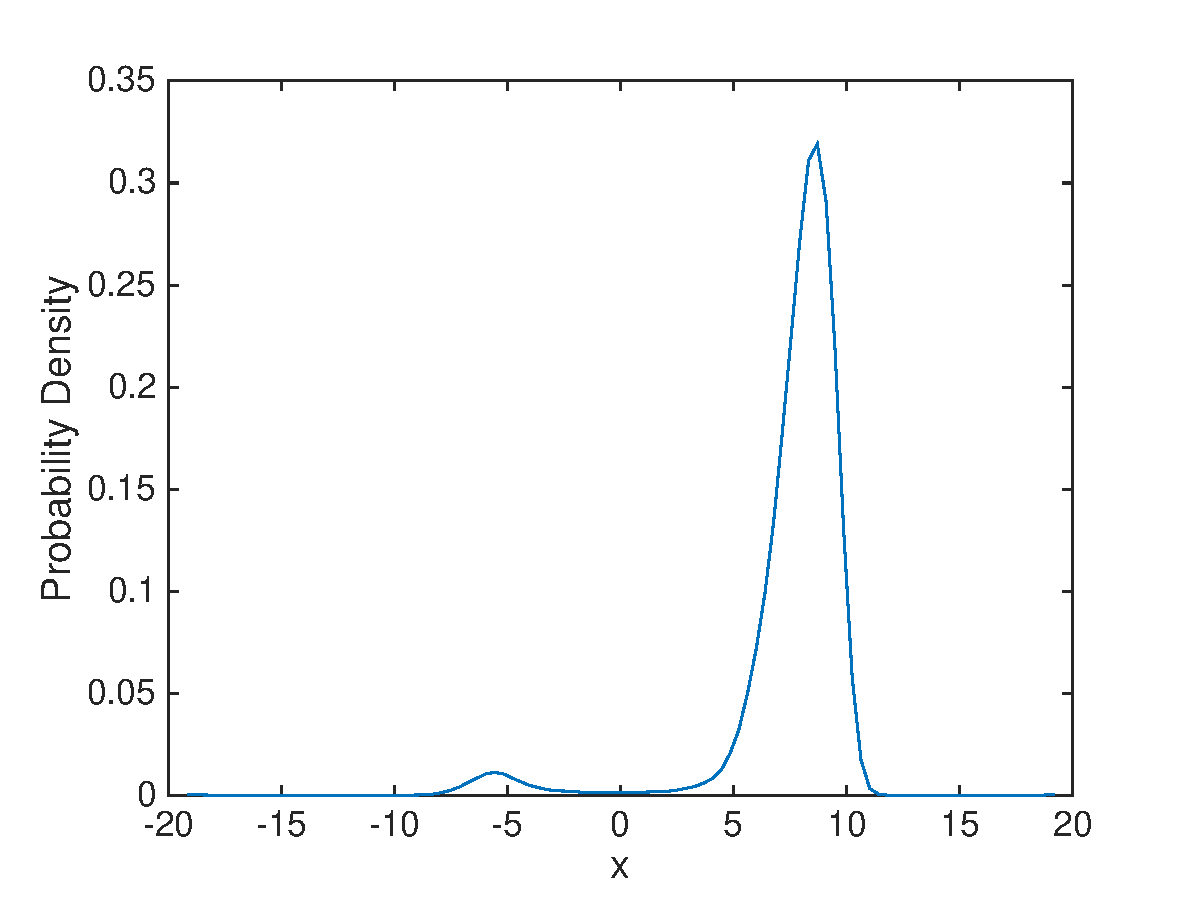
\includegraphics[width=0.3\textwidth]{figures/xhist}
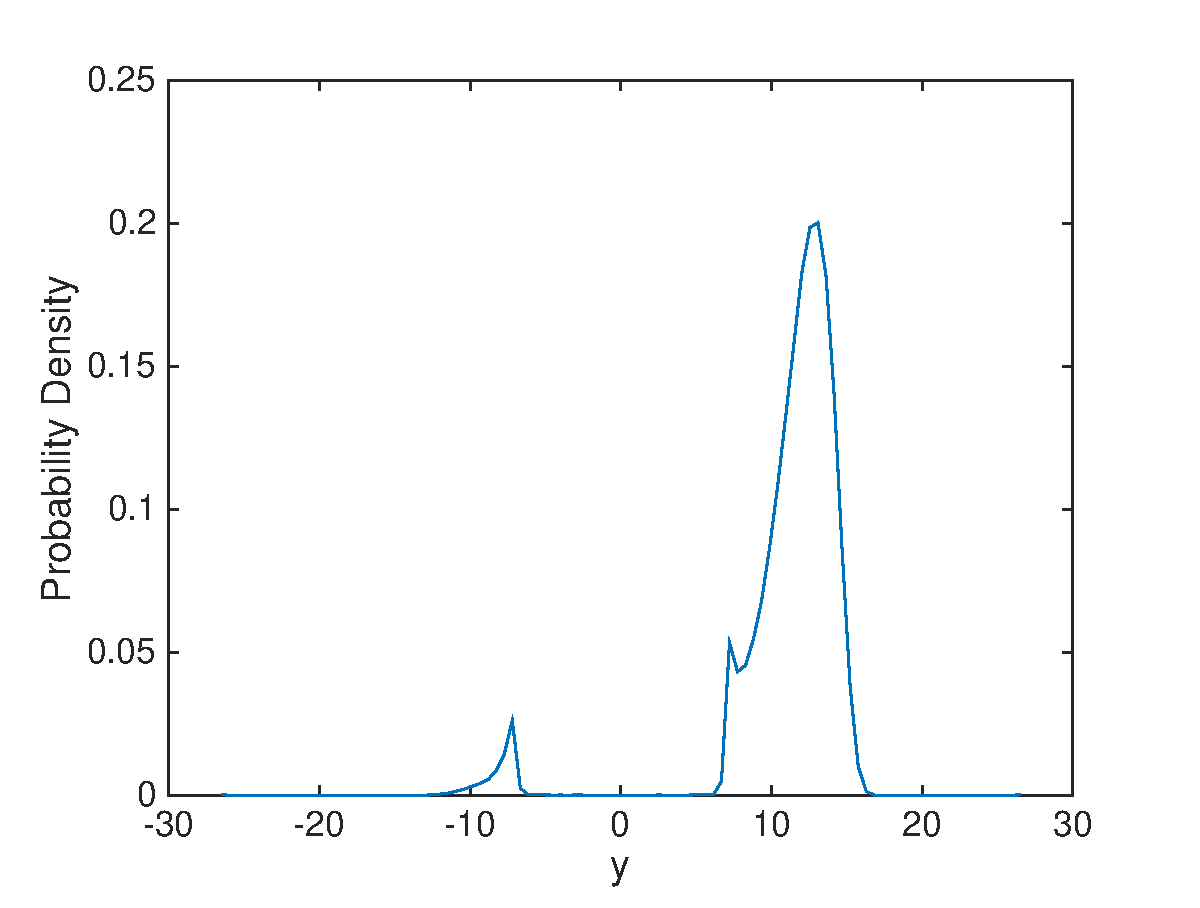
\includegraphics[width=0.3\textwidth]{figures/yhist}
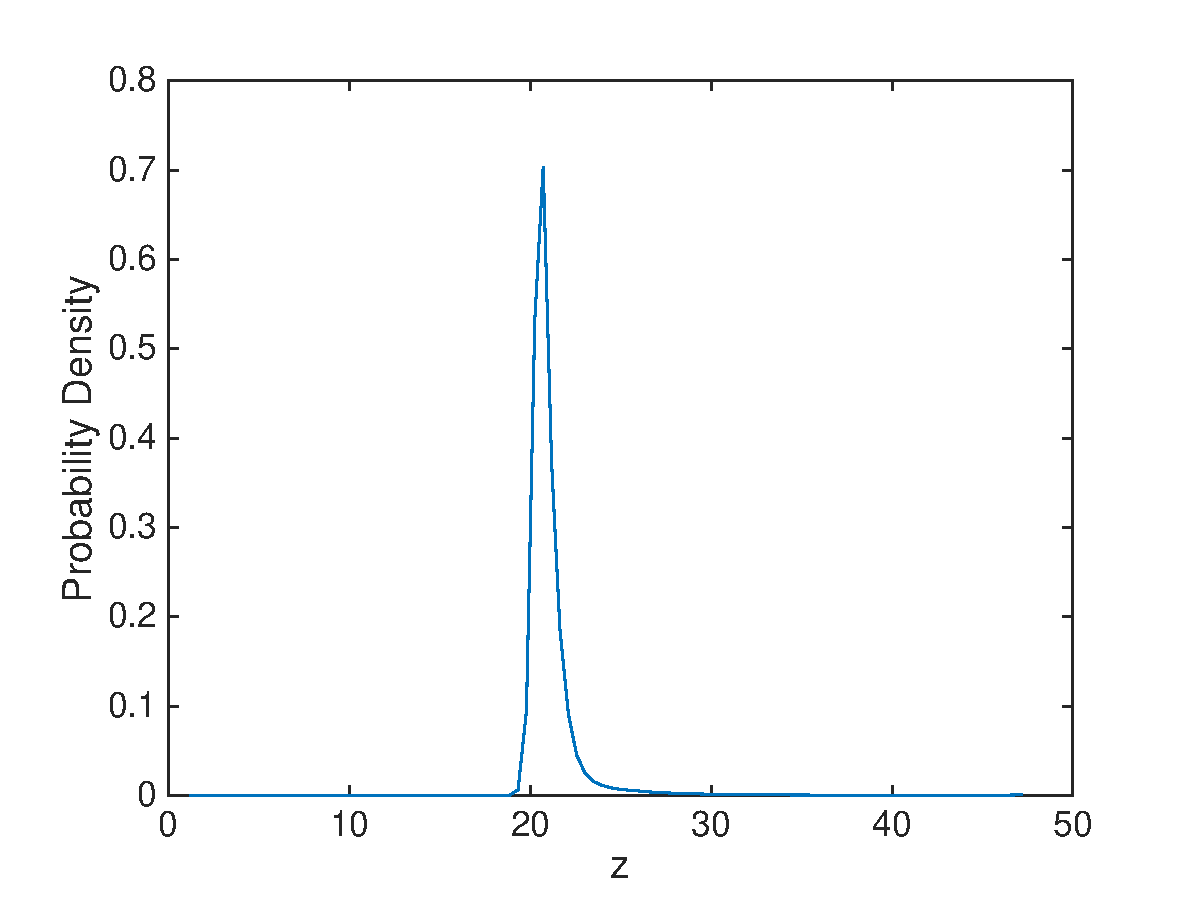
\includegraphics[width=0.3\textwidth]{figures/zhist}
\caption{Histograms from 1e7 Monte Carlo runs of the push forward of the new prior for the Lorenz '63 problem}
\end{figure}

The more dimensions and posterior complexity that exists in a problem, the bigger the ensemble will need to be to have a stable ETAIS implementation. After a certain point, due to the extra overheads with a large ensemble due to for example the resampling, ETAIS will no longer be competitive. This said, in our most recent work, arbitrarily complex posteriors can be efficiently sampled using ETAIS if used in conjunction with a transport map to simplify the target. This is the subject of our next paper which we will be submitting imminently. We have added a paragraph to this end to the discussion.}


  \comment{8) Do not use an explicit Euler solver, use any higher order, off the shelve solver.}{Many of the off-the-shelf higher order solvers are just as inappropriate to use for the approximation of the solution of the Lorenz '63 equations. We agree that the explicit Euler method with a small timestep is not an optimal choice, but it is a simple choice, which still leads to a chaotic nonlinear system. We argue that it is sufficient for the purpose of comparing the efficiency of two different Monte Carlo methods, both of which are using the same approximation of the likelihood.}

  %{Many of the off-the-shelf higher order solvers are just as inappropriate to use for the approximation of the solution of the Lorenz '63 equations, since they are chaotic, and as such \emph{any} numerical error is quickly amplified through the dynamics. Moreover, the focus of this paper is not on these applications, but in the statistical algorithm. In this example, we are simply looking for a non-linear mapping such that we can demonstrate the speed-up that is gained from using ETAIS as opposed to standard M-H sampling, and we believe that a simple Euler approximation provides such a mapping.}
\end{document}
